\begin{lemma}
    $m^*$ is translation-invariant.
\end{lemma}
\begin{proof}
    If we translate the set, we can translate all of its 
    covers as well. Since translating an interval does not
    change its length, the lengths of the covers won't change either.
\end{proof}

\begin{proposition}[Countable subadditivity]
    \label{the:countableSubadditivity}
    For any countable collection of sets
    $\{E_k\}_{k=1}^\infty$ we have 
    \[ m^*\Bigl(\bigcup_{k=1}^\infty E_k\Bigr) \le \sum_{k=1}^\infty m^*(E_k) \]
\end{proposition}
\begin{remark}
    We don't ask for the sets $E_k$ to be disjoint. 
    If we proved that we have an equality sign for the disjoint case,
    we would have proved that $m^*$ is a measure, which we proved does not exist
    in Theorem~\ref{the:measureNotExists}.
\end{remark}
\begin{proof}
    Choose open intervals $I_{k,i}$, such that
    \[E_k \subset \bigcup_{i=1}^\infty E_{k,i} \text{ ($E_{k, i}$ are a cover of $E_k$)}\] and
    \[\sum_{i=1}^\infty l(I_{k,i}) < m^*(E_k) + \frac{\varepsilon}{2^k}\]
    Such intervals exist from the definition of the infimum.

    On the other hand, $\{ I_{k,i} \mid 1 \le k, i < \infty \}$
    covers each of the $E_k$, and thus it's a cover of
    $\cup_{k=1}^\infty E_k$.
    Then 
    \[ 
        m^*\Bigl(\bigcup_{k=1}^\infty E_k\Bigr) \overset{\text{it's a cover}}{\le}
        \sum_{1 \le k, i < \infty} l(I_{k,i}) <
        \sum_{k=1}^\infty m^*(E_k) + \varepsilon \Bigl(\frac{1}{2} + \frac{1}{4} + \dots\Bigr) =
        \sum_{k=1}^\infty m^*(E_k) + \varepsilon
    \]
    Now take $\varepsilon \to 0$.
\end{proof}
\begin{remark}
    Here we assume that all of the $E_k$ have finite outer measures.
    Otherwise, both of the sides of the inequality would diverge
    to infinity, and we get $\infty \le \infty$ which is ``true''.
\end{remark}

\pagebreak
\subsection{The $\sigma$-algebra of Lebesgue-measurable sets.}
\begin{definition}
    A set $E$ is (Lebesgue) measurable if for any set 
    $A$,
    \[ 
        m^*(A) = m^*(A \cap E) + m^*(A \cap E^{C})
        \qquad E^C = \mathbb{R} \setminus E
    \]
    \begin{figure*}[h]
        \centering
        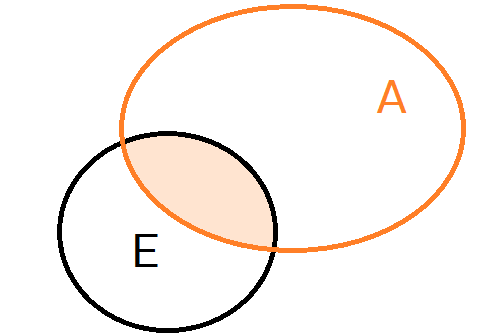
\includegraphics[width=0.3\textwidth]{measure_e_and_a}
        \caption{The set $E$ ``splits'' $A$ into two parts}
    \end{figure*}
\end{definition}
\begin{remark}
    We already have the $\le$ sign from Proposition~\ref{the:countableSubadditivity}.
\end{remark}
\begin{remark}
    Motivation: If $A \cap B = \emptyset$ and $A$ (or $B$) is measurable, then
    \[
        m^*(A \cup B) = m^*\bigl((A \cup B) \cap A\bigr) +
        m^*\bigl( (A \cup B)  \cap A^C \bigr) = m^*(A) + m^*(B)
    \]
\end{remark}

\begin{proposition}
    If $m^*(E) = 0$, then $E$ is measurable.
\end{proposition}
\begin{proof}
    For all $A$ we have:
    \begin{align*}
        &
        m^*(A \cap E) \le m^*(E) = 0 \implies m^*(A \cap E) = 0
        \\&
        m^*(A) \ge m^*(A \cap E^C) = m^*(A \cap E) + m^*(A \cap E^C)
    \end{align*}
    As we noted earlier, the inequality in the other side follows from 
    Proposition~\ref{the:countableSubadditivity}.
\end{proof}

% TODO make it Proposition 2 as in the second proposition in subsection.
\begin{proposition}  
    If $E_1, \dots, E_n$ are measurable, then 
    $\cup_{1}^n E_k$ is measurable.
\end{proposition}
\begin{proof}
    Case $n=2$:
    for all $A$ we have
    \begin{align*}
        &
        m^*(A) = m^*(A \cap E_1) +  m^*(A \cap E_1^C)
        =\\&=
        m^*(A \cap E_1) + m^*\bigl((A \cap E_1^C) \cap E_2\bigr) +
        m^*\bigl((A \cap E_1^C) \cap E_2^C\bigr) = (*)
        \\&
        X := A \cap E_1,\
        Y := (A \cap E_1^C) \cap E_2,\
        Z := (A \cap E_1^C) \cap E_2^C
    \end{align*}
    With Venn diagrams it's possible to prove that 
    $Z = A \cap (E_1 \cup E_2)^C$, $X \cup Y = A \cap (E_1 \cup E_2)$.
    Now let's apply Proposition~\ref{the:countableSubadditivity} to $X$ and $Y$. Then we get:
    \[
        (*) \ge m^*\bigl(A \cap (E_1 \cup E_2)\bigr) +
        m^*\bigl(A \cap (E_1 \cup E_2)^C\bigr)
    \]

    Induction step:
    Apply case $n=2$ to the sets 
    $\cup_{1}^{n - 1} E_k$, $E_n$.
\end{proof}